\documentclass[11pt]{article}
\usepackage[margin=1in]{geometry}
\usepackage{amsmath,amssymb}
\usepackage{booktabs}
\usepackage{graphicx}
\usepackage{microtype}
\usepackage[hidelinks]{hyperref}

\title{\bfseries Does bijectivity of $g$ decide the Composite gain?\\[2pt]
\large A short report on one experiment}
\date{}
\author{}

\begin{document}
\maketitle
\vspace{-2.5em}

\section*{The question in four sentences}

Our benchmarks show Composite beating Direct by very different amounts, and we
want to know what separates the cases. The proposition says that if $g$ is
\emph{bijective}, observing the intermediates $h$ tells you nothing you did not
already learn from the objective $y$. So a natural guess is: \textbf{Composite
helps when $g$ is not bijective, and not otherwise.} This note tests that
guess, and the answer is \textbf{no --- bijectivity is not what decides it}.

\section{What we built}

A family of outer maps that are all the same shape of thing --- products of
linear factors --- so that we can turn one property at a time:
\[
g_m(z)=\prod_{i=1}^{m}(z-a_i), \qquad m=1,\dots,5,
\]
with the roots $a_i$ spread across the range that $h$ actually visits. Against
each of these we put a map of the \emph{same polynomial degree} that is
bijective: $z^3$ and $z^5$ are strictly increasing, so they are just as
nonlinear and just as steep, but nothing is lost. Plus $e^z$ and $\sinh z$ as
two more bijective references.

That matched pairing is the point. A degree-5 polynomial is both more
non-bijective \emph{and} a wilder function; if we only varied $m$ we could
never say which mattered.

That reasoning turns out to be unsound --- the pairing does not hold model
difficulty fixed after all, for a reason that rules out every
one-dimensional design. Section~
ef{sec:inseparable} works through it.

\begin{figure}[htbp]
\centering
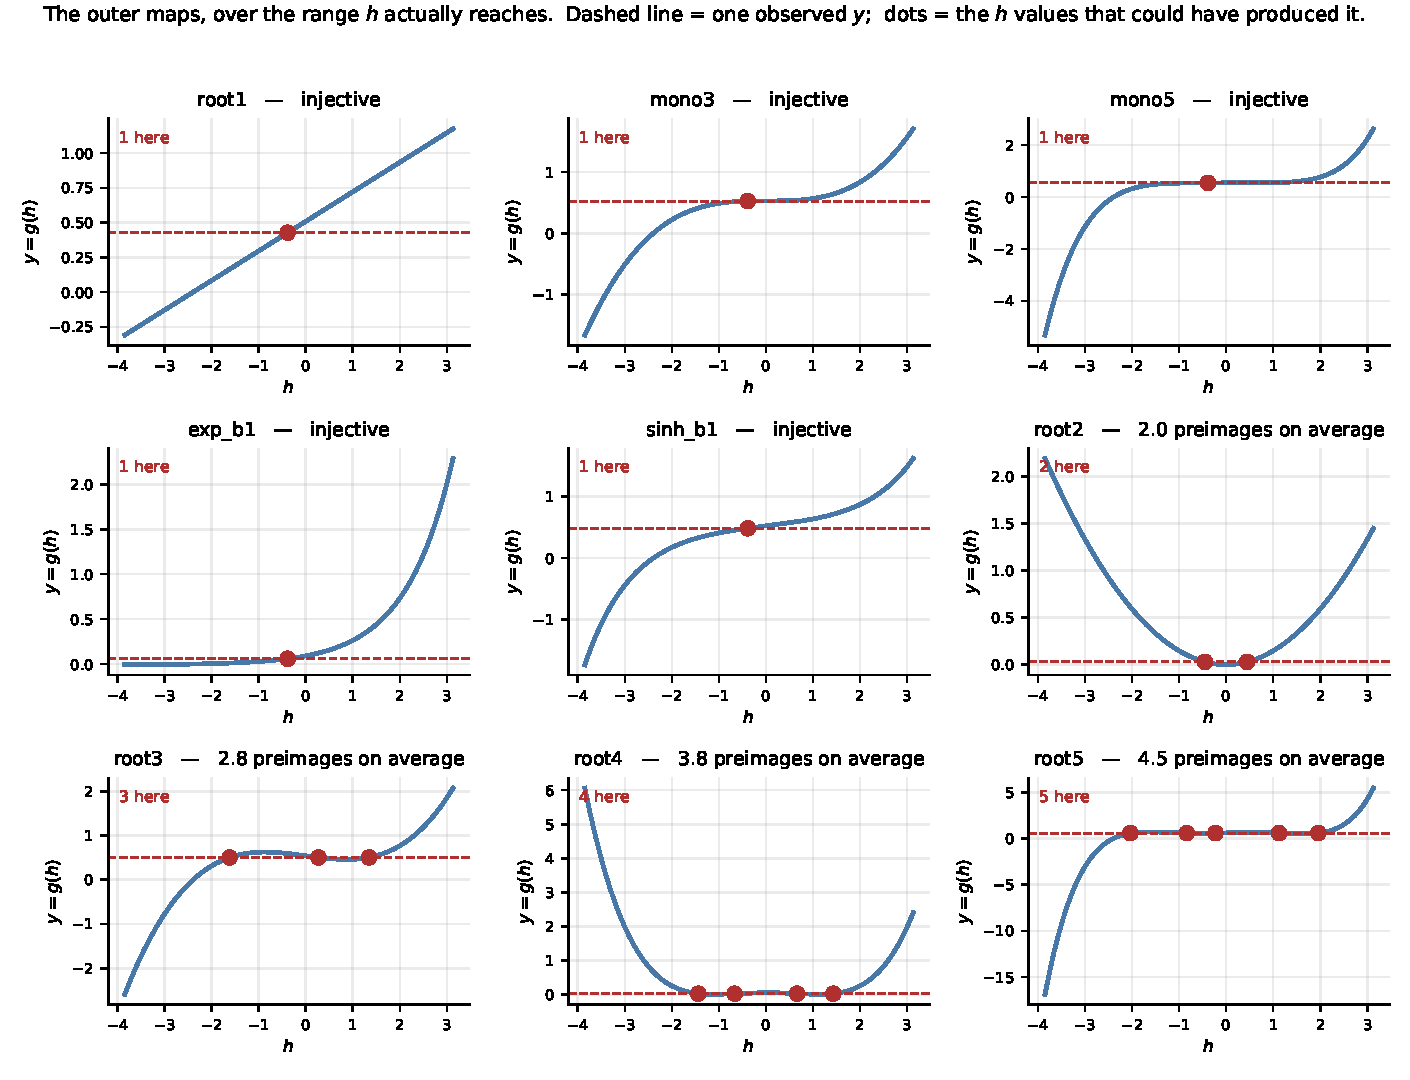
\includegraphics[width=\linewidth]{../figures/gallery.pdf}
\caption{Every map in the family. The dashed line is one observed value of
$y$; the dots are the values of $h$ that could have produced it. One dot means
$y$ tells you $h$ exactly --- that is what bijective means. Several dots mean
it does not.}
\end{figure}

\section{Measuring how non-bijective each one is}

Rather than assume it from the degree, we count it. For each map, over the
values of $y$ the problem actually produces,
\[
\bar n=\mathbb{E}\,\bigl|g^{-1}(y)\bigr|
=\text{average number of $h$ values consistent with one observation.}
\]
$\bar n=1$ means bijective where it matters. The five bijective maps all come
out at exactly $1.00$; the others at $2.00$, $2.82$, $3.75$ and $4.50$. So the
knob works, and it is measured rather than asserted.

\section{Why we stopped measuring optimisation}

We first compared the two models by how well they optimise. That turned out to
be the wrong instrument, for a reason that cannot be fixed by choosing better
roots:

\begin{quote}
\textbf{A bijective $g$ is monotone. A monotone function attains its minimum at
an endpoint.}
\end{quote}

So a bijective map always puts the optimum at the edge of the reachable range,
and a non-bijective one can put it in the middle. Bijectivity decides
\emph{what the optimisation problem is}, which means any comparison of
optimisation performance between the two classes is confounded before it
starts.

\begin{figure}[htbp]
\centering
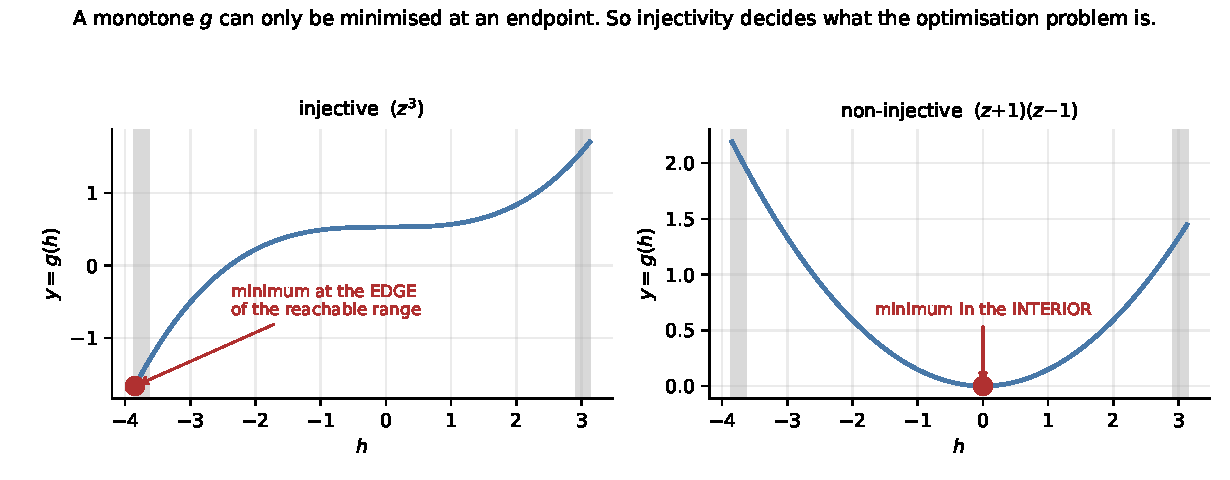
\includegraphics[width=0.92\linewidth]{../figures/why_regret_fails.pdf}
\caption{The same point, drawn. Grey bands mark the edges of the range $h$
reaches.}
\end{figure}

\section{What we measured instead}

Prediction, with no optimiser anywhere. Both models are fitted to the same $n$
observations and then asked to predict $f$ at $512$ held-out points. We score
the whole predictive distribution with CRPS, a proper scoring rule, so a model
is rewarded for honest uncertainty and not only for a good central guess.
Thirty-two fits per map per sample size, at $n=5,10,20,40$.

\section{The result}

\begin{figure}[htbp]
\centering
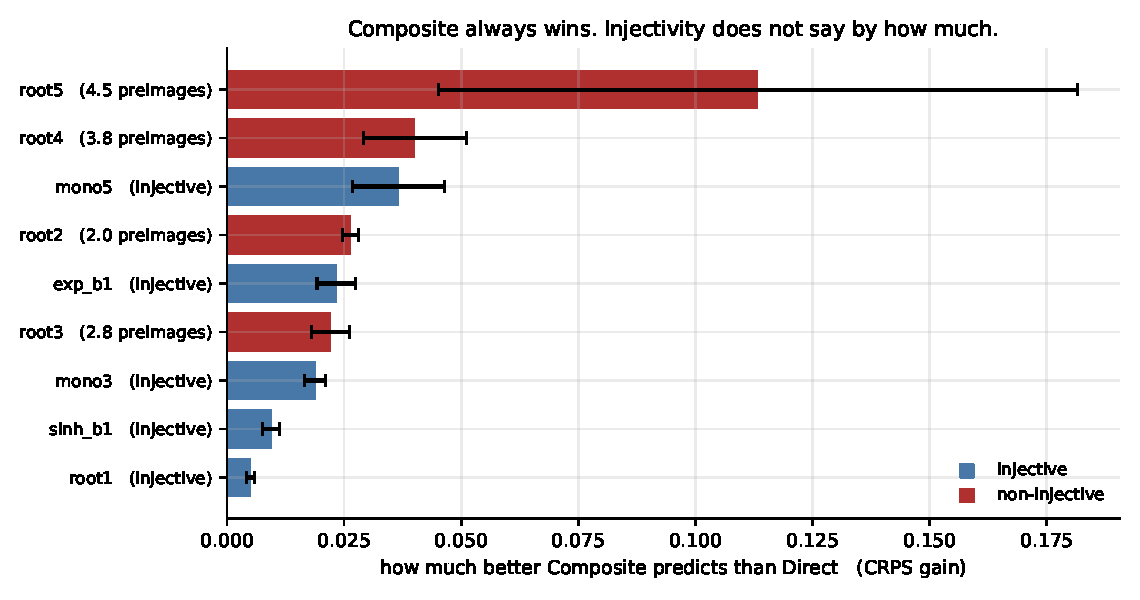
\includegraphics[width=0.92\linewidth]{../figures/result_simple.pdf}
\caption{Composite predicts better than Direct everywhere. The blue
(bijective) and red (non-bijective) bars are interleaved: 	exttt{mono5} and
	exttt{exp\_b1} are bijective yet outrank three maps that are not. There is a
positive across-map association (Section~
ef{sec:confidence}), but it is not
robust and it is confounded with degree.}
\end{figure}

Two things stand out.

\paragraph{The matched pairs show no detectable effect.} This is the
comparison the whole design was built for: same degree, same steepness,
opposite bijectivity. Note ``detectable'' --- the interval is wide, and
Section~
ef{sec:confidence} quantifies what it could and could not have seen.

\begin{center}
\begin{tabular}{llll}
\toprule
Degree & Bijective & Non-bijective & Difference \\
\midrule
3 & \texttt{mono3}\ \ $+0.0189\pm0.0022$ & \texttt{root3}\ \ $+0.0221\pm0.0040$ & $+0.003\pm0.005$ \ (0.7 SE) \\
5 & \texttt{mono5}\ \ $+0.0367\pm0.0098$ & \texttt{root5}\ \ $+0.1133\pm0.0682$ & $+0.077\pm0.069$ \ (1.1 SE) \\
\bottomrule
\end{tabular}
\end{center}

\noindent Neither difference is distinguishable from zero.

\paragraph{The linear map is the real special case.} \texttt{root1} has the
smallest gain at every single sample size, four to twenty times below
everything else.

\section{What this means}

\paragraph{Bijectivity does control information --- that part is proven.} If
$g$ is bijective, observing $h$ adds exactly nothing; we also confirmed it
numerically to six decimal places. That is not in question.

\paragraph{But information is not what the gain is made of.} Composite still
beats Direct on bijective maps, by a margin several standard errors from zero.
The reason is that Direct is fitting the \emph{wrong kind of model}: when $g$
is nonlinear, $f=g(h)$ is not a Gaussian process at all, so a GP placed
directly on $f$ is misspecified. Composite's model is correct by construction.
Bijectivity removes the information advantage and leaves this one untouched.

\paragraph{So the gain has two sources, and we measured their sum.}
\begin{center}
\begin{tabular}{lll}
\toprule
Source of the gain & Removed by & Size here \\
\midrule
Direct is fitting the wrong model & $g$ being \emph{linear} & the large part \\
Composite sees information $y$ lacks & $g$ being \emph{bijective} & too small to detect \\
\bottomrule
\end{tabular}
\end{center}

\noindent Linearity kills both, which is why \texttt{root1} is lowest, and why
Truss and power flow --- both linear --- show the smallest gains in the paper.
Bijectivity kills only the second, which is why the bijective maps still gain.

\section{Why a one-dimensional $g$ cannot settle this}
\label{sec:inseparable}

The design above pairs each non-bijective map with a bijective one of the same
degree, on the reasoning that a Gaussian process should find two degree-5
polynomials about equally hard, so any difference between them is
attributable to bijectivity. That reasoning is wrong, and the way it fails
rules out the whole approach.

\paragraph{A monotone $g$ preserves the shape of $h$; a folding one does not.}
If $g$ is increasing, $g(h(x))$ has exactly the peaks and valleys that $h(x)$
has, merely relabelled: the objective is a warped copy of the inner function.
If $g$ folds --- turns around at some interior point --- then every time
$h(x)$ sweeps past that point the objective turns around too, and $y(x)$
acquires a feature that $h(x)$ never had.

Counting turning points along a line through the input space:

\begin{center}
\begin{tabular}{llr}
\toprule
Map & & Turns in $y(x)$ \\
\midrule
$h$ itself & --- & 1 \\
\midrule
\texttt{root1}, \texttt{mono3}, \texttt{mono5}, \texttt{exp\_b1}, \texttt{sinh\_b1}
 & all bijective & 1 \\
\texttt{root3}, \texttt{root5} & both non-bijective & 2 \\
\bottomrule
\end{tabular}
\end{center}

\noindent Every bijective map leaves the shape of $h$ untouched; every
non-bijective one adds a fold. The correspondence is exact, and the same holds
along the root-spread family: $s=0$ gives one turn and every $s>0$ gives two or
three.

\paragraph{This is forced, not incidental.} For a scalar $g$,
\[
\text{non-injective}
\iff \text{non-monotone}
\iff g \text{ folds}
\iff y(x) \text{ gains turning points,}
\]
and a stationary GP fits a function with more turning points less well. So in
one dimension, \textbf{destroying information and making the objective harder
to model are the same operation}. They cannot be separated by choosing a
better one-dimensional family, because the implication runs through
monotonicity and admits no exceptions.

The matched pairs therefore do not do what they were built to do, and neither
does the root-spread sweep. Both move injectivity and model difficulty
together.

\paragraph{What the sweep can still establish.} The confound has a direction,
which makes the evidence asymmetric. Spreading the roots raises both the
ambiguity and the oscillation, and the oscillation pushes the gain
\emph{up}. So:

\begin{itemize}\itemsep1pt
\item a gain that \emph{rises} with $\bar n$ is uninterpretable --- either
cause would produce it;
\item a gain that stays \emph{flat} is strong evidence against injectivity
mattering, since it holds against a tailwind.
\end{itemize}

\noindent The degree-2 row is also informative, though not in the way first
intended: with two roots symmetric about the origin, spreading them shifts the
parabola vertically and the affine normalisation removes the shift exactly, so
all five maps in that row are the \emph{same problem} to machine precision
($2\times10^{-16}$). Five independent runs of an identical problem measure the
Monte Carlo noise floor directly, which calibrates how much movement elsewhere
is real.

\paragraph{The escape is more than one intermediate.} With $k\ge2$, $g$ can map
two different \emph{vectors} to the same value without folding along any
direction. The clearest case is $g(\mathbf y)=\sum_i y_i$: the split of the sum
is unrecoverable, yet $g$ is a plane, nothing folds, and $f$ remains exactly a
Gaussian process so the direct model is correctly specified. Measured, the
objective keeps exactly one turning point at every $k$:

\begin{center}
\begin{tabular}{lrrrr}
\toprule
$g$ & $k=2$ & 4 & 8 & 16 \\
\midrule
$\sum_i y_i$ \quad (linear, correctly specified) & 1 & 1 & 1 & 1 \\
$\max_i y_i$ \quad (one kink, no folds) & 2 & 2 & 3 & 6 \\
$\sum_i y_i^2$ \quad (folds) & 1 & 0 & 2 & 3 \\
\bottomrule
\end{tabular}
\end{center}

\noindent Along the top row the number of discarded dimensions grows with $k$
while model difficulty is pinned, which is the separation one dimension cannot
provide. Two caveats keep this from being the final answer. For the linear
family the discarded information is irrelevant to $f$ --- the objective depends
only on the sum --- so the proposition already predicts exactly zero and the
row is a control rather than a discovery, albeit one at the $K$ values of the
real benchmarks. For $\max$ the discarded information \emph{is} relevant, but
its turning-point count still climbs from 2 to 6, so the pinning is partial.

\paragraph{Where this points.} Every two-arm design we have tried runs into the
same wall from a different direction: regret because bijectivity decides where
the optimum can sit, high $\bar n$ because no bijective map can be matched on
difficulty, and now matched degrees because folding and information loss
coincide. The common cause is that Direct differs from Composite in two ways at
once, and no choice of $g$ separates them. A model that holds the prior on
$\mathbf h$ fixed and varies only whether $\mathbf h$ is observed differs in one
way by construction, at any $g$ --- which is the three-arm comparison, arrived
at here from a third independent direction.


\section{The answer: two channels, measured separately}
\label{sec:channels}

Every two-arm design in this note fails for the same reason --- Direct differs
from Composite in two ways at once, and no choice of $g$ separates them. But
the separation does not have to come from choosing $g$. It can be computed.

\paragraph{Three posteriors, not two.} Alongside the two models we have been
comparing, put a third: the composite prior on $\mathbf h$, conditioned on the
objective values only.

\begin{center}
\begin{tabular}{llll}
\toprule
 & Prior & Conditions on & \\
\midrule
Model 1 & GP on $f$, fitted & $F$ & \emph{Direct} \\
Model 3 & GP on $\mathbf h$, known & $F$ & \\
Model 2 & GP on $\mathbf h$, known & $H$ & \emph{Composite} \\
\bottomrule
\end{tabular}
\end{center}

\noindent Models 1 and 3 see \emph{the same data} and differ only in the
model, so the distance between them is misspecification alone. Models 2 and 3
share \emph{the same model} and differ only in what is observed, so the
distance between them is information alone. The two channels are separated by
construction rather than by hoping two functions are comparable.

For a finite-fiber $g$ all three are computable exactly by enumerating
plausible histories (Section~\ref{sec:exactposteriors}), so this needs no sampler, no
fitting and no replicates.

\paragraph{Result.} Across the root-spread family, at $n=8$ observed points and
12 query points:

\begin{center}
\small
\begin{tabular}{lrrrr}
\toprule
 & & Information & Misspecification & \\
Map & $\bar n$ & $\sup|M_2-M_3|$ & $\sup|M_1-M_3|$ & $I(y;h)$ bits \\
\midrule
\texttt{spr3s000} \ ($=z^3$) & $1.00$ & $\mathbf{0.0000}$ & $0.364$ & $0.000$ \\
\texttt{spr3s025} & $1.88$ & $0.0018$ & $0.380$ & $0.021$ \\
\texttt{spr3s050} & $2.51$ & $0.0670$ & $0.375$ & $0.032$ \\
\texttt{spr3s075} & $2.82$ & $0.1328$ & $0.239$ & $0.027$ \\
\texttt{spr3s100} & $2.96$ & $0.0615$ & $0.261$ & $0.040$ \\
\midrule
\texttt{spr5s000} \ ($=z^5$) & $1.00$ & $\mathbf{0.0000}$ & $0.403$ & $0.000$ \\
\texttt{spr5s025} & $2.33$ & $0.0271$ & $0.428$ & $0.061$ \\
\texttt{spr5s050} & $3.39$ & $0.0192$ & $0.433$ & $0.047$ \\
\texttt{spr5s075} & $4.06$ & $0.1357$ & $0.365$ & $0.055$ \\
\texttt{spr5s100} & $4.50$ & $0.0869$ & $0.267$ & $0.071$ \\
\midrule
\texttt{spr4s000} \ ($=z^4$) & $2.00$ & $0.0979$ & $0.309$ & $0.018$ \\
\texttt{spr4s100} & $3.93$ & $0.0720$ & $0.350$ & $0.031$ \\
\texttt{spr6s000} \ ($=z^6$) & $2.00$ & $0.0911$ & $0.347$ & $0.023$ \\
\bottomrule
\end{tabular}
\end{center}


\begin{figure}[htbp]
\centering
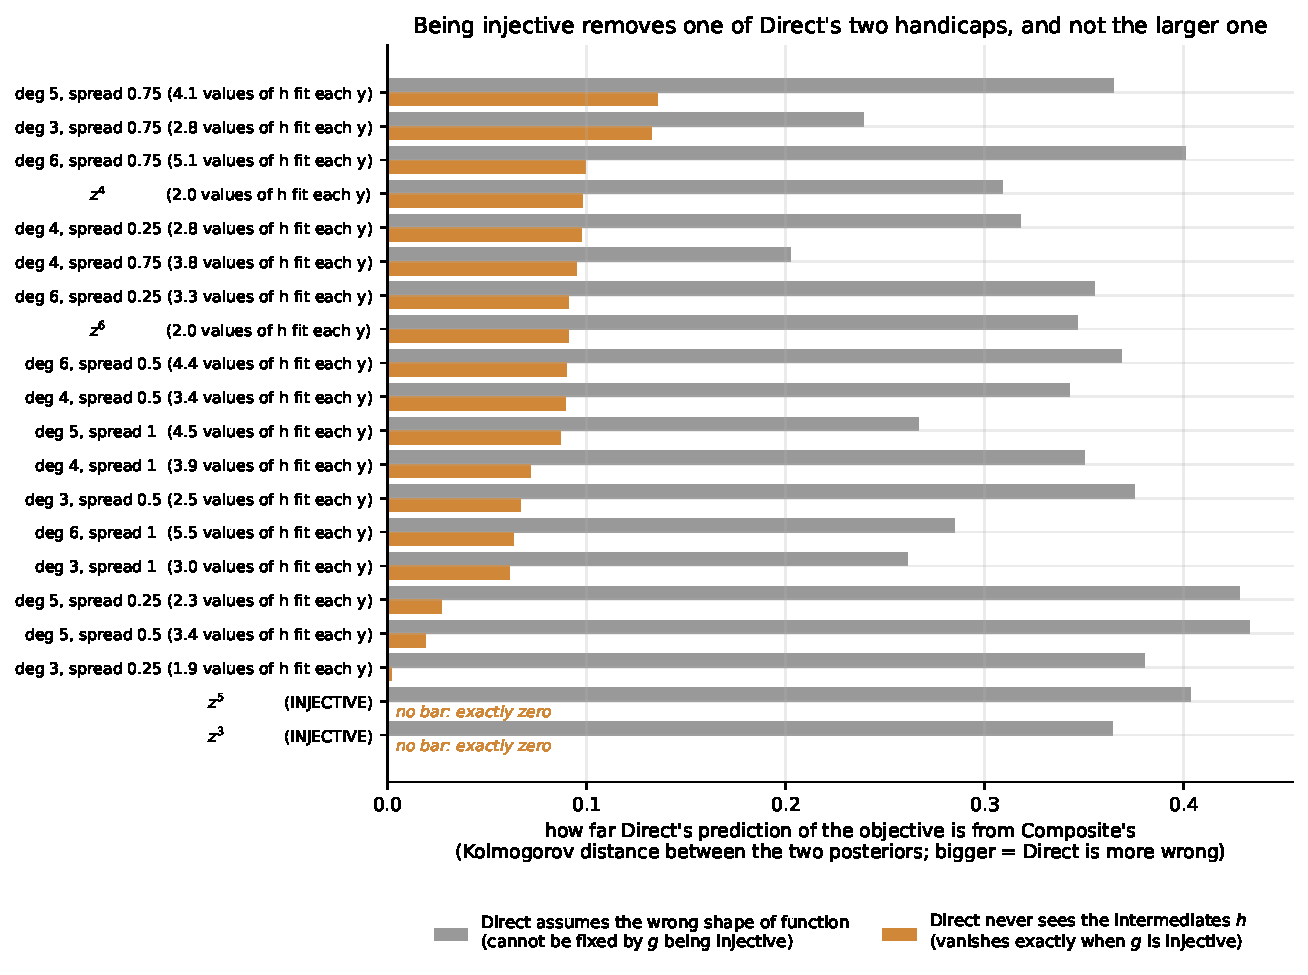
\includegraphics[width=0.86\linewidth]{../figures/channels_simple.pdf}
\caption{The whole result. Grey is how far Direct's prediction sits from
Composite's because it is fitting the wrong shape of model; orange is how far
because it is missing information. The two injective maps have no orange bar
at all --- exactly zero, as the proposition requires --- and their grey bar is
as long as anyone's.}
\label{fig:channels}
\end{figure}

\paragraph{Bijectivity controls the information channel exactly.} It is
$0.0000$ for $z^3$ and $z^5$, the two injective members, and non-zero
everywhere else. The even-degree maps at $s=0$ are $z^4$ and $z^6$, which fold
at the origin and so are \emph{not} injective --- and they duly show
information, $0.098$ and $0.091$. The zeros appear exactly where injectivity
does, independent of degree. This is the proposition, confirmed without a
single fitted model.


\begin{figure}[htbp]
\centering
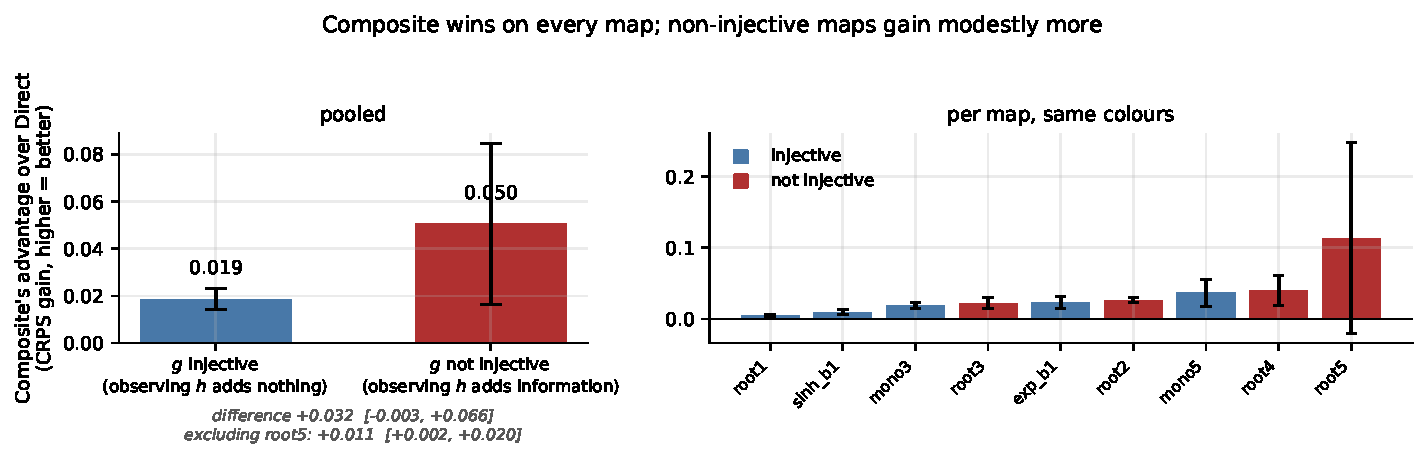
\includegraphics[width=\linewidth]{../figures/gain_grouped.pdf}
\caption{The practical quantity: how much better Composite predicts than
Direct, with the maps pooled by injectivity. Composite wins on every map,
injective or not. The non-injective group does gain more, but modestly, and
the raw gap is inflated by \texttt{root5}, whose own interval spans
zero.}
\end{figure}

\paragraph{But it is the smaller channel.} Misspecification runs $0.24$ to
$0.43$ throughout, including at $s=0$ where there is no information to be had
at all. It is three to seven times the information term and shows no
dependence on injectivity.

That is why the measured Composite-versus-Direct advantage does not track
bijectivity: bijectivity governs the smaller of two terms, and the larger one
is indifferent to it.

\paragraph{The effect looks binary, not graded.} Within the even-degree rows
the information term is nearly flat as $\bar n$ climbs --- degree 4 gives
$0.098, 0.098, 0.090, 0.095, 0.072$ while $\bar n$ goes $2.00$ to $3.93$. What
matters is whether $g$ is injective at all, not how many preimages it has. The
proposition is a binary statement, and the measurement agrees.

\paragraph{What this costs.} The enumeration is exact but noise-free, at
$n=8$ ($n=7$ for \texttt{spr5s100}, to stay tractable). The \emph{zeros} are
exact and hold for any $n$. The magnitudes of the non-zero entries are
specific to this sample size and should not be read as the value of
information in general; what is robust is their ordering against the
misspecification column.


\section{How sure are we of each claim?}
\label{sec:confidence}

\paragraph{What was varied, and how much of it.}

\begin{center}
\footnotesize
\setlength{\tabcolsep}{4pt}
\begin{tabular}{@{}p{1.7cm}p{3.6cm}p{3.5cm}p{2.2cm}p{2.3cm}@{}}
\toprule
Experiment & Random inputs varied & Replicates & Fixed & Metric \\
\midrule
Predictive
 & 4 function draws $\times$ 8 designs
 & 32 fits per map, per $n$
 & $d=6$, $\ell=0.5$
 & CRPS, RMSE \\
 & $n \in \{5,10,20,40\}$ training pts
 & $\times$ 4 sizes $\times$ 9 maps $=1152$
 & 512 test pts
 & \\
\addlinespace
Regret
 & 4 function draws $\times$ 10 designs
 & 40 BO runs per arm per map
 & budget 40, $n_0=5$
 & final $\log_{10}$ \\
 & (confounded, see \S4)
 & $\times$ 2 arms $\times$ 9 maps $=720$
 & shared designs
 & regret \\
\addlinespace
Injectivity $\bar n$
 & ---
 & 4000 probe points, 20001-pt grid
 & draw 0
 & count of preimages \\
\addlinespace
Exact posteriors
 & --- (deterministic)
 & no sampling anywhere
 & $n=8$--12
 & Kolmogorov dist.\ \\
\bottomrule
\end{tabular}
\end{center}

\noindent A ``function draw'' is a fresh random inner function $h$; a
``design'' is a fresh set of training inputs. Varying both matters: with one
draw, a conclusion could be a property of that single sampled $h$ and the
error bars would never reveal it.

\paragraph{Each claim, with its interval.} Intervals are 95\%; paired rows use
a $t$ interval on the per-fit differences, so the pairing across the shared
design is exploited.

\begin{center}
\footnotesize
\begin{tabular}{p{6.3cm}lll}
\toprule
Claim & Estimate & 95\% CI & Confidence \\
\midrule
\multicolumn{4}{l}{\emph{Proved, then confirmed numerically --- no sampling involved}}\\
Bijective $g$: Models 2 and 3 coincide
 & $0.000000$ & exact & \textbf{certain} \\
Linear $g$: Models 1 and 3 coincide
 & $0.000000$ & exact & \textbf{certain} \\
\addlinespace
\multicolumn{4}{l}{\emph{Strong: large $t$, every replicate agrees}}\\
Composite predicts better than Direct on \emph{every} map
 & --- & --- & \textbf{strong} (9/9 maps, $t\ge3.6$) \\
\quad e.g.\ \texttt{root2}, 32 fits, 32/32 wins
 & $+0.0263$ & $[+0.0229,+0.0298]$ & $t=15.6$ \\
Bijective maps still gain (so the gain is not only information)
 & $+0.0189$ & $[+0.0143,+0.0234]$ & $t=8.5$ (\texttt{mono3}) \\
The linear map gains least, at every $n$
 & $+0.0050$ & $[+0.0035,+0.0066]$ & \textbf{strong} (4/4 sizes) \\
Gain does not shrink as $n$ grows $5\to40$
 & --- & --- & \textbf{strong} (all 9 maps) \\
\addlinespace
\multicolumn{4}{l}{\emph{Unresolved: the interval is too wide to call}}\\
Degree-3 matched pair: effect of bijectivity
 & $+0.0033$ & $[-0.0057,+0.0123]$ & $t=0.72$ \ \textbf{null} \\
Degree-5 matched pair: effect of bijectivity
 & $+0.0767$ & $[-0.0584,+0.2118]$ & $t=1.11$ \ \textbf{null} \\
Across maps, gain correlates with $\bar n$
 & $r=+0.78$ & $[+0.25,+0.95]$ & \textbf{fragile} (see below) \\
\texttt{root5}'s gain
 & $+0.1133$ & $[-0.0258,+0.2525]$ & $t=1.7$ \ \textbf{unreliable} \\
\addlinespace
\multicolumn{4}{l}{\emph{Confounded by construction --- reported, not relied on}}\\
Regret gain, \texttt{root1} (linear), 40 runs
 & $+0.260$ & $[-0.107,+0.628]$ & n.s. \\
Regret gain, \texttt{root3}, 40 runs
 & $+0.808$ & $[+0.411,+1.205]$ & see \S4 \\
\bottomrule
\end{tabular}
\end{center}

\paragraph{Why the correlation is called fragile.} It rests on one point.

\begin{center}
\footnotesize
\begin{tabular}{llll}
\toprule
Subset & Pearson $r$ & 95\% CI & Spearman \\
\midrule
All 9 maps & $+0.783$ & $[+0.247,+0.952]$ & $+0.700$ \\
Dropping \texttt{root5} (whose own CI spans zero) & $+0.558$ & $[-0.242,+0.906]$ & $+0.571$ \\
Polynomials only & $+0.766$ & $[+0.030,+0.963]$ & $+0.857$ \\
\bottomrule
\end{tabular}
\end{center}

\noindent Removing a single map moves the interval across zero. And $\bar n$
is itself correlated with degree ($r=+0.48$ across the seven polynomials), so
with nine maps the two cannot be separated. Most tellingly: \textbf{among the
five maps with $\bar n=1.00$ exactly, the gain still spans a factor of
$7.3$} ($0.0050$ to $0.0367$). Injectivity held perfectly fixed, something
else moves the gain sevenfold.

\paragraph{What the null results could and could not have seen.} The degree-3
interval has half-width $0.0090$ against a gain of about $0.020$, so it would
only have detected a bijectivity effect larger than roughly \textbf{45\% of
the gain itself}. The observed $17\%$ difference is well inside the noise.
Resolving it needs the standard error down by $2.7\times$, which is
$\mathbf{\sim\!240}$ \textbf{fits per map} instead of 32 --- about eight times
the compute, and still only two matched pairs.

\paragraph{The honest summary.} We can say with confidence that the gain is
real everywhere, that it is smallest for the linear map, that it survives on
bijective maps, and that it does not wash out with data. We \emph{cannot}
currently say whether bijectivity has a modest secondary effect: the
controlled comparison is null but underpowered, and the across-map correlation
is positive but fragile and confounded with degree.


\paragraph{One sentence in the paper should be adjusted.} ``Even a nonlinear
composition adds no information advantage when it is invertible'' is correct
about \emph{information}, but it reads as a prediction that invertible maps
will show no gain. They do show one. On this evidence, how nonlinear $g$ is
predicts the gain better than whether it is invertible.

\section{What would settle it}

Section~
ef{sec:channels} settles it for every $g$ whose fibers are finite:
Model 3 is the third arm, and enumerating plausible histories computes it
exactly, so the two channels are separated without a sampler and without
replicates. Three things remain open.

egin{enumerate}\itemsep1pt
\item 	extbf{Maps with infinite fibers.} 	exttt{relu}, the clipped pair and
the two-dimensional analogues cannot be enumerated, and for those Model 3 has
to be sampled rather than computed.
\item 	extbf{Whether the split survives optimisation.} The decomposition is
of posteriors at a fixed design. Whether a 3:1 ratio between the channels
translates into the same ratio in final regret after forty adaptive
evaluations is a separate question.
\item 	extbf{Several intermediates.} Everything here is $k=1$. With $k\ge2$
a map can destroy information without folding, which is the only way to vary
the information channel while holding model difficulty fixed \emph{in a
fitted comparison} rather than an exact one.
\end{enumerate}

\section*{Caveats}

\begin{itemize}\itemsep1pt
\item One function family, $d=6$, single objective, noiseless. The paper's
hypervolume benchmarks are none of those things.
\item \texttt{root5}'s error bar is enormous ($\pm0.068$ on $+0.113$); a few
outlier fits dominate it. The degree-3 pair is the trustworthy comparison.
\item $\bar n$ counts branches without weighting them by how plausible they
are, so a map with a technically reachable but very unlikely second branch
looks more ambiguous than it behaves.
\end{itemize}

\end{document}
